\section{Multi-case Comparison}
\label{ch:multicase}

Several analysis modules support importing CSV files from previous \href{https://cmdrryder.github.io/uPrime/}{uPrime} sessions and overlaying them on top of the current plot. This is useful for comparing experimental conditions, validating against numerical data, or assembling multi-panel publication figures.

The same workflow is used in: Mean \& Convergence (Mean Velocity tab), Reynolds Stress, TKE Budget, Spectra (Spatial Welch and Temporal), Correlation, and Anisotropy (Lumley line mode).

\subsection{Importing a case}

Click `Import Case\ldots` and select a CSV file. The CSV must follow the column layout produced by \href{https://cmdrryder.github.io/uPrime/}{uPrime}'s own `Export Profile` or `Export Data` actions. The imported case is added to the case list with an auto-assigned color and dashed linestyle.

\begin{figure}[htbp]
  \centering
  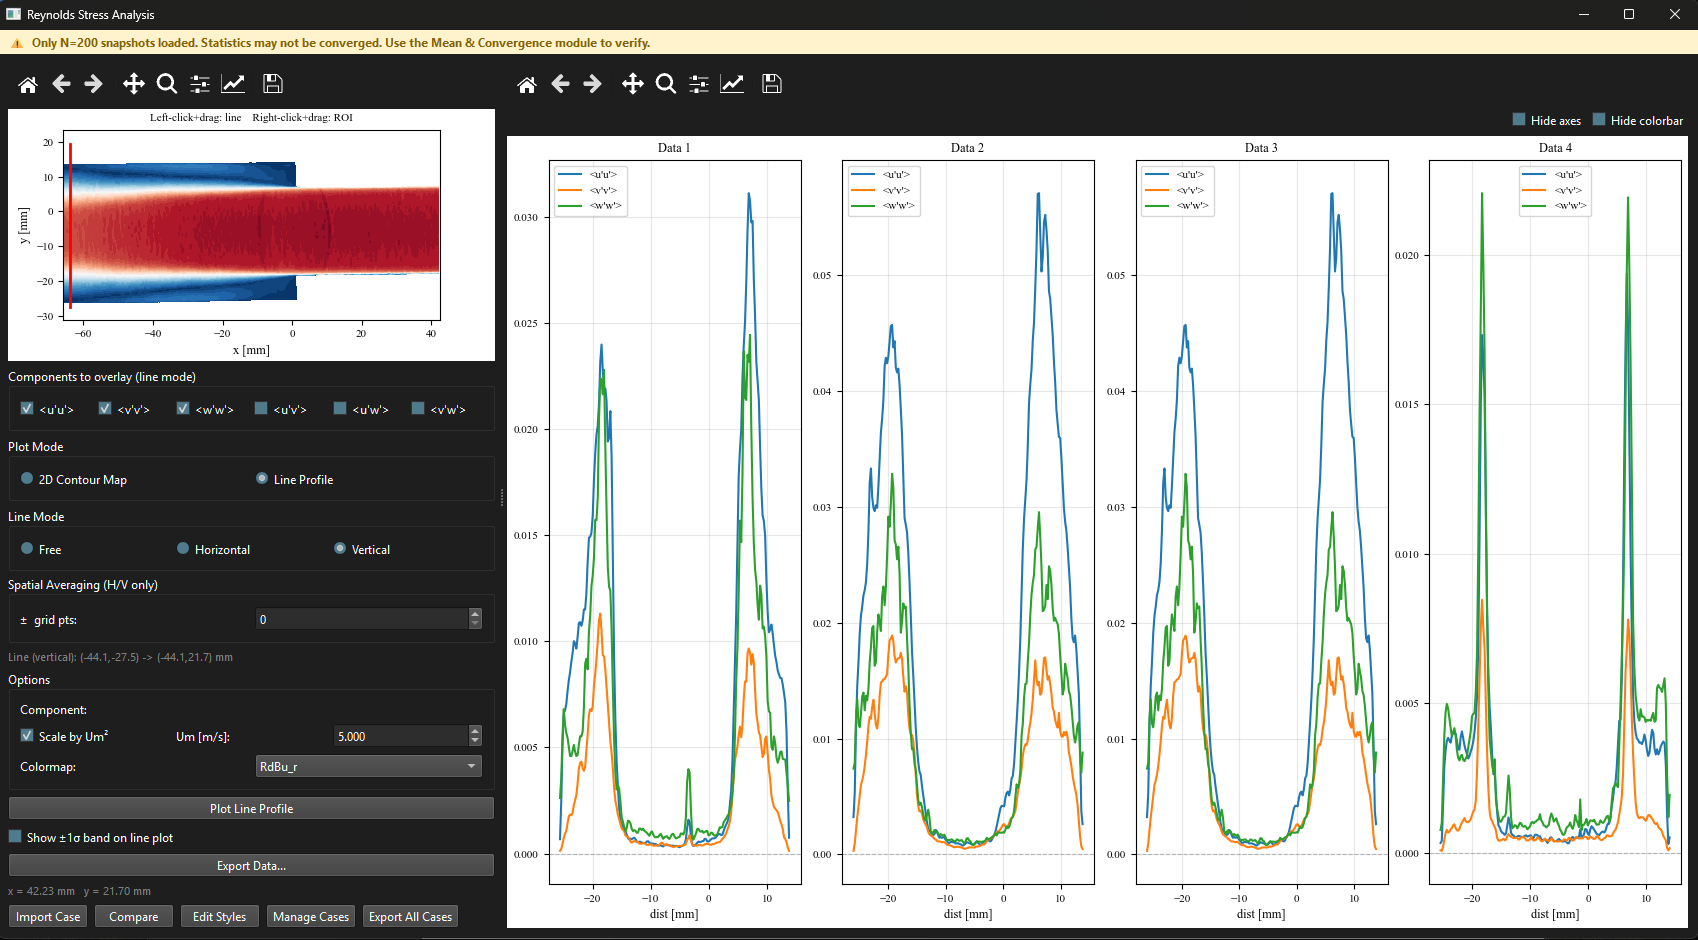
\includegraphics[width=0.92\linewidth]{fig_multicase_overlay}
  \caption{Reynolds stress line profile with two imported cases overlaid. The current dataset is shown as solid lines; imported cases use distinguishable colors and linestyles. The legend uses the user-assigned label per case.}
  \label{fig:multicase}
\end{figure}

\subsection{Managing cases}

Click `Manage Cases\ldots` to open the Case Manager dialog. From here, cases can be renamed, hidden, or removed. Each case retains its imported file path, line geometry (where applicable), and any header metadata such as $U_m$.

\begin{figure}[htbp]
  \centering
  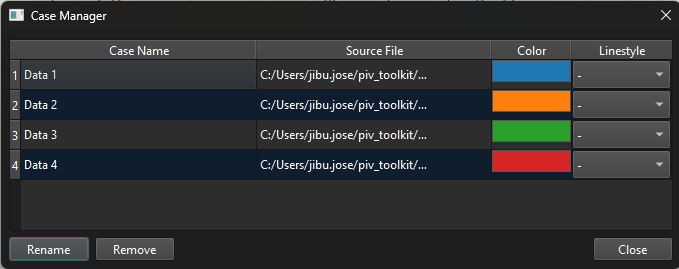
\includegraphics[width=0.55\linewidth]{fig_case_manager}
  \caption{Case Manager dialog. Each row corresponds to one imported case. Use the rename field to change the legend label; toggle visibility with the checkbox; click `Remove` to drop a case from the list.}
  \label{fig:casemgr}
\end{figure}

\subsection{Plot styles}

Click `Edit Styles\ldots` to change line color, linestyle, marker, and label per case. The current dataset and imported cases are styled independently.

\subsection{Quantity selector and layout chooser}

For modules with multiple quantities (Reynolds stresses with several components, TKE budget with $P$, $C$, $D$, $R$, etc.), the quantity selector controls which quantity is overlaid. The layout chooser switches between single-axes overlay and a faceted grid (one panel per case, sharing axes).

\subsection{Combined export}

Click `Export All Cases\ldots` to save the current dataset and all visible imported cases together in a single CSV. A \texttt{case} column is added to identify which row belongs to which case, suitable for pandas, MATLAB, or further plotting.

\subsection{Header consistency checks}

\href{https://cmdrryder.github.io/uPrime/}{uPrime} reads metadata from CSV headers when available. For Mean Velocity profiles, the \texttt{\# U\_m =} header is read per imported case. If the imported $U_m$ differs from the current setting, a status-bar warning is shown for that specific case so you can manually re-normalize before publishing.

\begin{quote}
\textbf{Warning}
\href{https://cmdrryder.github.io/uPrime/}{uPrime} does not automatically convert units between cases. If your imported CSV uses different units (mm vs m, m/s vs U/U\_m, etc.), the comparison will be misleading. Check the header values and re-export the source data in a consistent format if needed.
\end{quote}

% ============================= CHAPTER 15 ==============================
